\documentclass{lug}
\usepackage{graphicx}
\usepackage{amsmath}
\usepackage{bm}
\usepackage{color}

\title[H-Nets]{Harmonic Networks: Deep Translation and Rotation Equivariance}
\author{Daniel E. Worrall, Stephan J. Garbin, Daniyar Turmukhambetov and Gabriel J. Brostow}
\institute[CSM]{\textbf{Presented By:} \\ Lou Brand \\ Department of Computer Science\\Colorado School of Mines}
\date{\today}

\begin{document}

\section{Motivation}
\frame{
    \frametitle{Current Convolutional Neural-Network Implementation}
    \begin{itemize}
        \item<1-> CNNs are designed to map an image to a feature
            vector $$\bm{I}(\bm{x}) \xrightarrow{f} f(\bm{I}) $$
        \item<2-> When the image is translated then the feature vector coming out
            of the CNN is a \textit{proportionally-translated} version of the same
            feature vector
        \begin{center}
            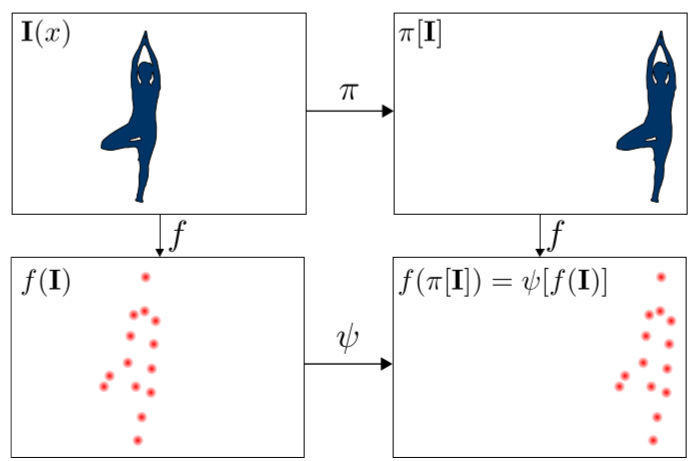
\includegraphics[scale=.3]{images/fig1.png}
        \end{center}        
    \end{itemize}
}

\frame{
    \frametitle{Current Convolutional Neural-Network Implementation}
    \begin{itemize}[<+->]
        \item Key Observations:
        \begin{enumerate}
            \item Translational equivariance has been 'baked-in' to the architecture of current CNN models
            \item CNNs learn the \textit{correlations between pixels}
            \item This feature extraction strategy hurts performance CNNs with rotated images 
        \end{enumerate}
        \item Current Soltuions:
        \begin{enumerate}
            \item "Aggressive Data Augmentation"
            \begin{itemize}
                \item Wastes computation during the training phase
                \item A rotated image is treated differently than it's non-rotated counterpart
            \end{itemize}
        \end{enumerate}
    \end{itemize}
}

\section{Intuition}
\frame{
    \frametitle{Imaginary Numbers}
    \begin{center}
        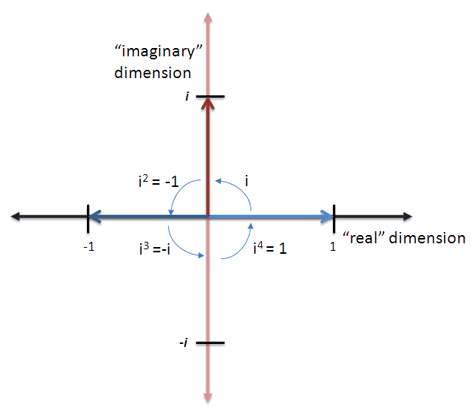
\includegraphics[scale=.5]{images/imaginary_cycle.png}
    \end{center}
}

\frame{
    \frametitle{Complex Numbers}
    \begin{center}
        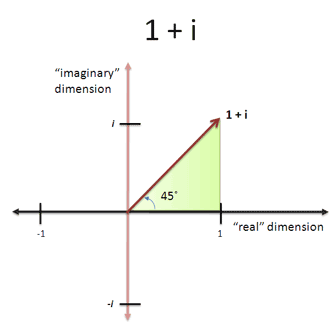
\includegraphics[scale=.65]{images/one_plus_i.png}
    \end{center}
}

\frame{
    \frametitle{Example}
    \begin{center}
        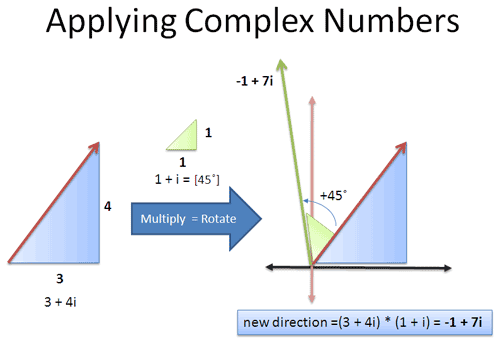
\includegraphics[scale=.60]{images/imaginary_example2.png}
    \end{center}
}



\section{Harmonic Networks}

\frame{
    \frametitle{Introducing Harmonic Networks}
    \begin{itemize}
    \item[] Feature mapping follows: $ \bm{W}_m(r, \phi; R, \beta) = R(r)e^{i(m\phi+\beta)} $
    \begin{columns}[T]
        \begin{column}{.5\textwidth}
            \begin{block}{Example}
                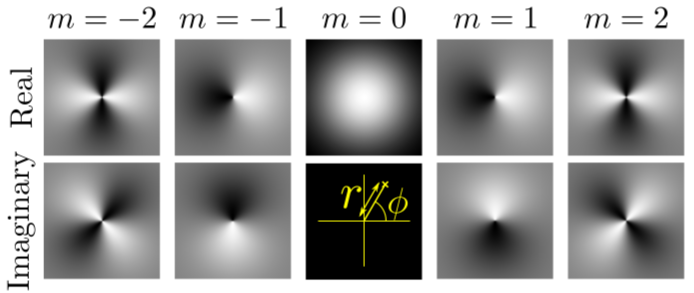
\includegraphics[width=.95\textwidth]{images/fig2.png}
                $$ R(r) = e^{-r^2} $$
                $$ \beta = 0 $$
            \end{block}
        \end{column}
        \begin{column}{.5\textwidth}
            \begin{block}{Key}
                \pause
    \item[] $ r, \phi $ coordinates of the image in polar coordinates.
        \pause
    \item[] $ m \in \mathbb{Z} $ is the rotation order
        \pause
    \item[] $ R(r) $ is the \textit{radial profile}. This controls the shape of the filter. Learned during training.
        \pause
    \item[] $ \beta \in [0, 2\pi] $ gives filter orientation selectivity. Learned during training. 
            \end{block}
        \end{column}
    \end{columns}
    \end{itemize}
}

\frame{
    \frametitle{Equivariance}
    \begin{itemize}
    \item[] \textbf{Key Insight:} $ [\bm{W} \star \bm{F}(r, \phi - \theta)] = e^{im\theta}[\bm{W} \star \bm{F}(r, \phi)] $ 
    \begin{center}
        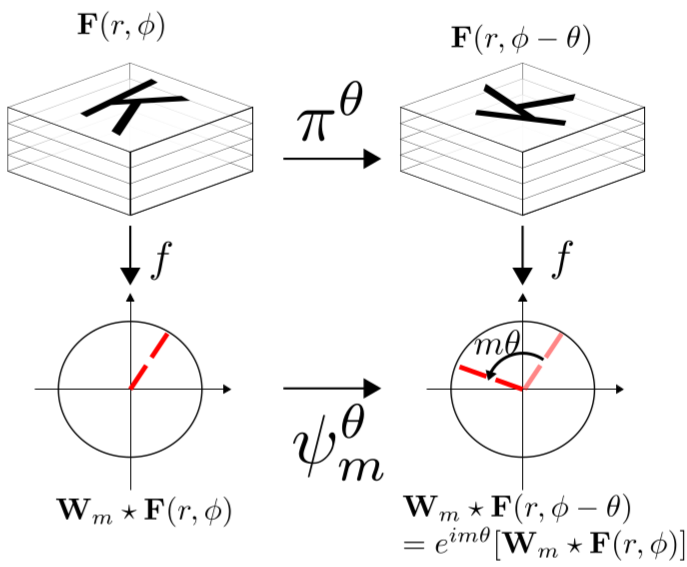
\includegraphics[scale=.3]{images/fig3.png}
    \end{center}
    \end{itemize}
}

\frame{
    \frametitle{Equivariance: Proof}
    Assume $ \bm{W}_m = R(r)e^{i(m\phi+\beta)} $ and $ \phi' = \phi - \theta $
    \begin{align*}
        [\bm{W} \star \bm{F}(r, \phi - \theta)] &= \int \bm{W}(r, \phi) \bm{F}(r, \phi - \theta)drd\phi \\ 
        &= \int \bm{W}(r, \phi' + \theta) \bm{F}(r, \phi')drd\phi' \\
        &= \int R(r)e^{i(m(\phi'+\theta)+\beta)}\bm{F}(r,\phi')drd\phi'\\
        &= e^{im\theta} \int R(r)e^{i(m\phi'+\beta)}\bm{F}(r,\phi')drd\phi'\\
        &= e^{im\theta}[\bm{W} \star \bm{F}(r, \phi)] 
    \end{align*}
    It follows that cross-correlation with $ \bm{W}_m $ yields a 360$^\circ$ rotationally equivariant feature mapping.
}

\frame{
    \frametitle{Structure}
    \begin{center}
        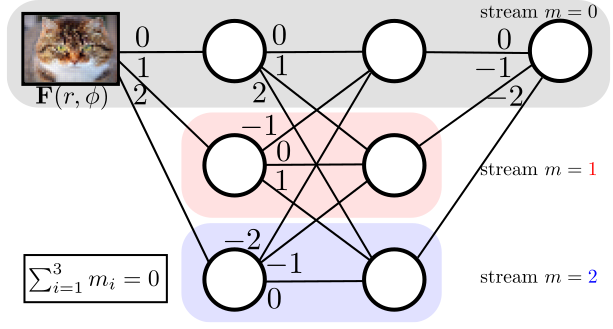
\includegraphics[scale=1]{images/fig4.png}
    \end{center}
    Edges represent cross-correlations with the rotation order of the corresponding filter ($ \bm{W}_m $). The sum of rotation orders must equal $ M = 0 $ to maintain \textit{rotational equivariance} in the Harmonic Network. Authors use the term "disentanglement."
}

\frame[shrink=7]{
    \frametitle{Equivariance: Chained Cross-Correlation}
    \begin{align*}
        \bm{W}_n(\hat{r},\hat{\phi}) \star [\bm{W}_m(r, \phi) \star \bm{F}(r, \phi - \theta)] &= \bm{W}_n(\hat{r},\hat{\phi}) \star e^{im\theta} [\bm{W}_m \star \bm{F}](\hat{r}, \hat{\phi} - \theta)\\ 
        &= e^{im\theta}(\bm{W}_n(\hat{r}, \hat{\phi}) \star [\bm{W}_m \star \bm{F}](\hat{r}, \hat{\phi} - \theta))\\ 
        &= e^{im\theta}e^{in\theta}[\bm{W}_n \star [\bm{W}_m \star \bm{F}]]\\
        &= e^{i(m+n)\theta}[\bm{W}_n \star [\bm{W}_m \star \bm{F}]]
    \end{align*}
    \pause
    We can see from this that chained cross-correlation results in the summation of the rotation orders of the individual filters $\bm{W}_m$ and $\bm{W}_n$. The above property determines the \textit{disentangled} structure observed in Harmonic Networks.\\ 
    \pause
    This property makes sure that at every feature map in the network the equivariance condition is maintained. Without this the responses from each filter ($\bm{W}$) will become \textit{entangled}. \textcolor{blue}{\href{images/rotating_spherical_harmonics.gif}{Intuition.}}
}

\newcommand{\hyphen}[1]{{\operatorname{#1}}}

\frame{
    \frametitle{Structure}
    \begin{center}
        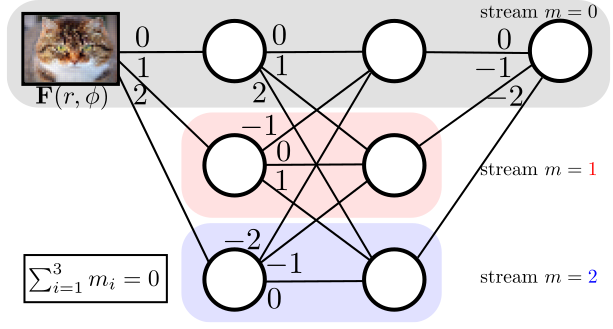
\includegraphics[scale=1]{images/fig4.png}
    \end{center}
    Between the cross-correlations with $\bm{W}$ the authors use a complex version of ReLU:
    $$ \hyphen{\mathbb{C}-} ReLU_b(Xe^{i\phi})=ReLU(X+b)e^{i\phi} $$
}

\section{Implementation}
\frame{
    \frametitle{Image Sampling}
    \begin{center}
        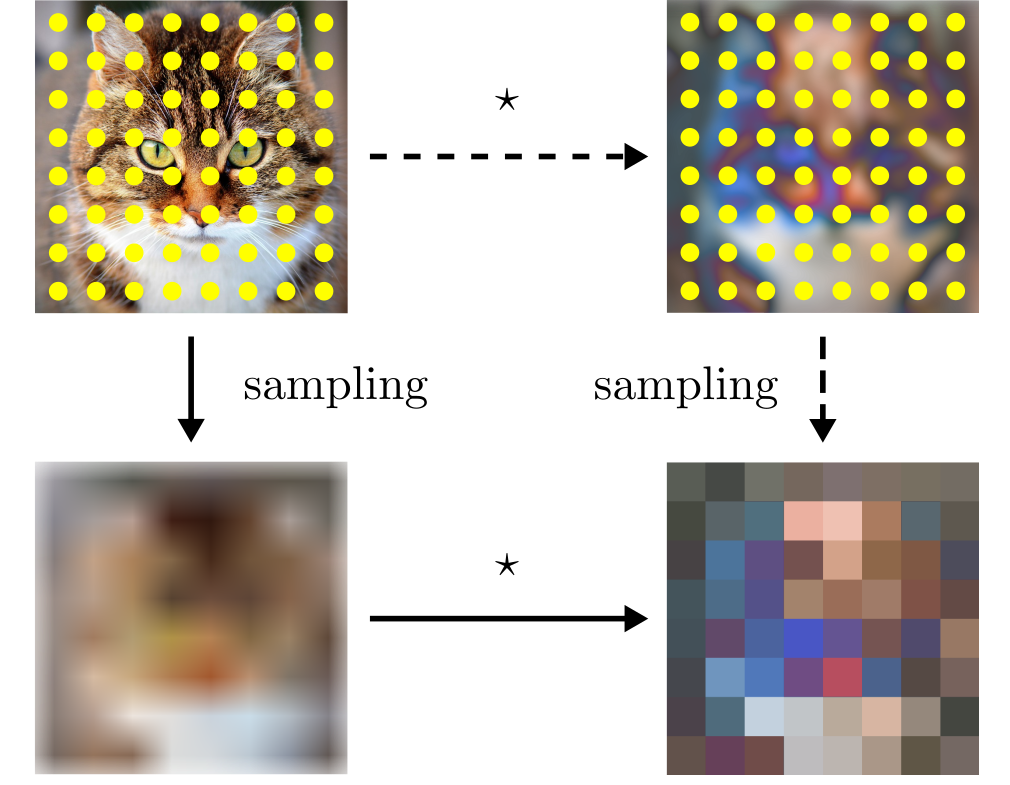
\includegraphics[scale=1]{images/fig5.png}\\
        Each yellow dot represents a \textit{center of equivariance}.\\
    \end{center}
    \pause
    \textbf{Key Insight:} Sampling and cross-correlation commute. The implementation path is chosen due to computaitonal complexity. 
}

\frame{
    \frametitle{Filter ($\bm{W}$) Implementation}
    \begin{center}
        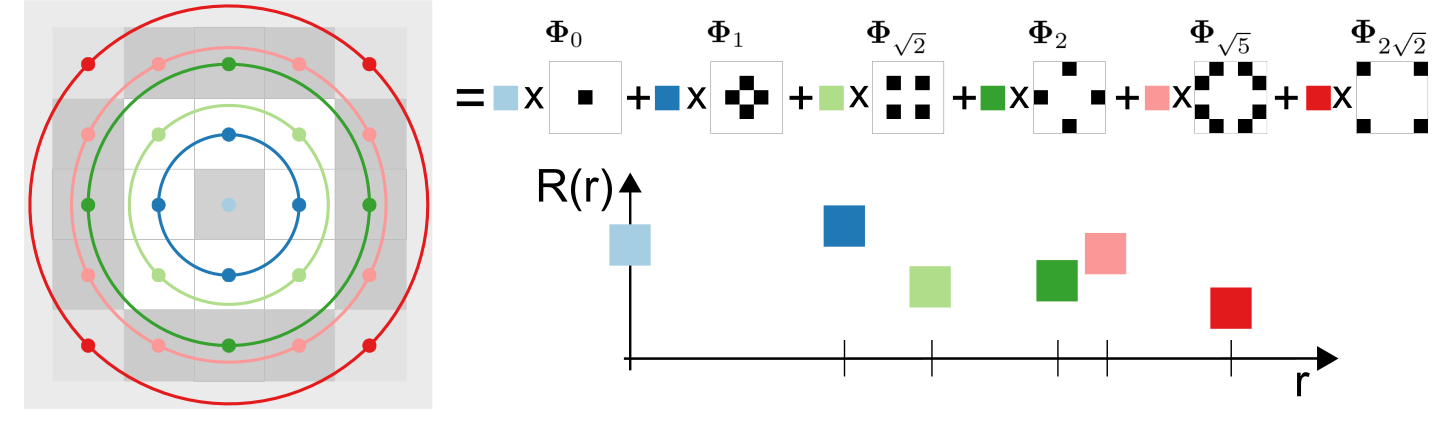
\includegraphics[scale=1]{images/fig6.png}\\
        Each matrix $\bm{\Phi}_{r_i}$ specifies elements equidistant from the center of the filter.
        \pause
        \begin{equation*} 
       	    \sum\limits_{i=1}^{I}\bm{R}(r_i)e^{i(m\bm{\Phi}_{r_i} + \beta)} = \sum\limits_{i=1}^{I}\bm{R}(r_i) 
       	    \begin{bmatrix}
       	        \bm{I}cos\beta & -\bm{I}sin\beta \\
       	        \bm{I}sin\beta & \bm{I}cos\beta           
       	    \end{bmatrix} 
            \begin{bmatrix}
                cos m\bm{\Phi}_{r_i} \\
                i sin m\bm{\Phi}_{r_i}
            \end{bmatrix}
        \end{equation*}
        \pause
        $\bm{R}(r_i)$ weights and $\beta$ are learned during training.
    \end{center}
}

\section{Experiments}

\frame{
    \frametitle{Structure}
    \begin{center}
        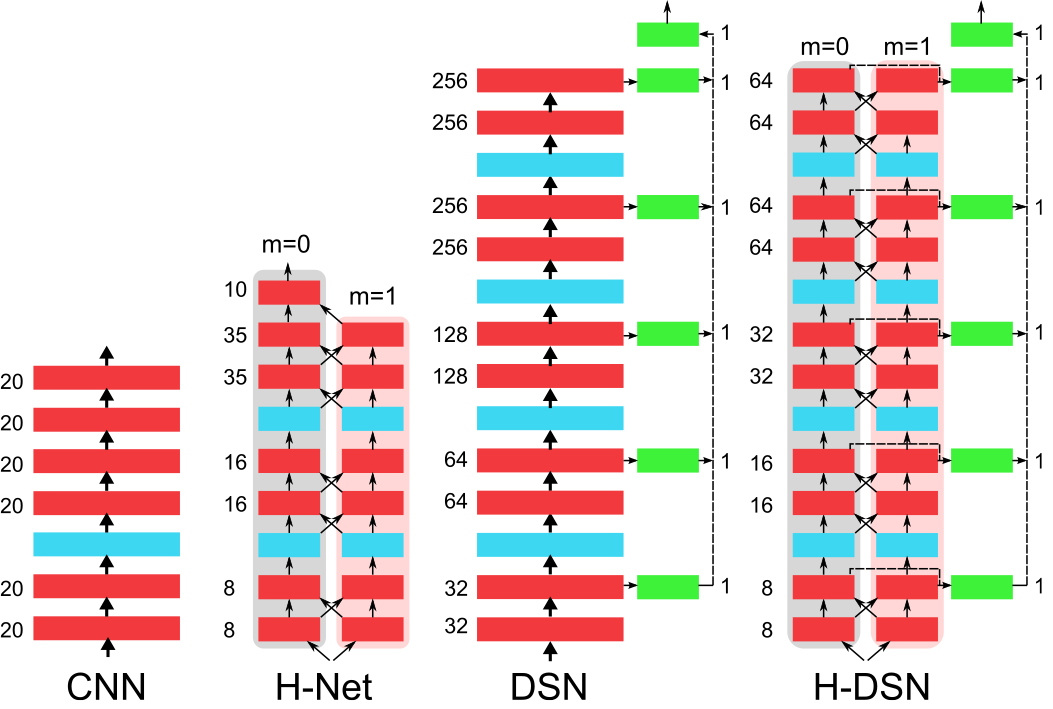
\includegraphics[scale=1]{images/fig7.png}
    \end{center}
}

\frame{
    \frametitle{Rotated MNIST}
    \begin{center}
        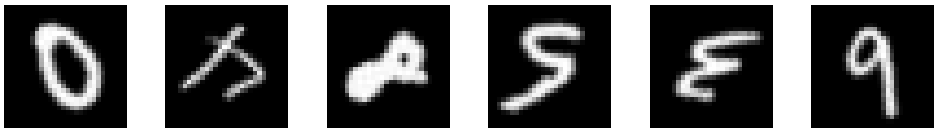
\includegraphics[scale=.5]{images/mnist-rot.png}\\
        \begin{tabular}{ |l|c|c| }
            \hline
            Method & Test Error (\%)&\# Parameters\\
            \hline
            \hline
            SVM & 11.11 & -\\
            Transformation RBM& 4.2 & -\\
            Conv-RBM & 3.98 & -\\
            CNN & 5.03 & 22k\\
            CNN + data aug& 3.50 &22k\\
            P4CNN rotation pooling& 3.21 & 25k\\
            P4CNN & 2.28 & 25k\\
            Harmonic Network & \textbf{1.69} & 33k\\
            \hline
        \end{tabular}
    \end{center}
}

\frame{
    \frametitle{Rotated MNIST}
    \begin{center}
        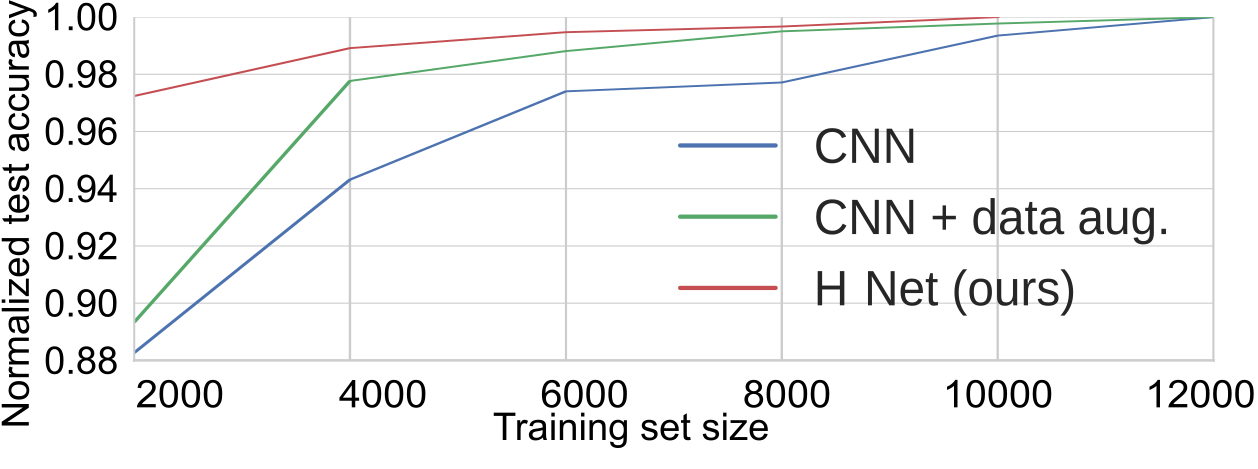
\includegraphics[scale=1]{images/fig9.png}\\
        Data efficiency of Harmonic Networks
    \end{center}
}

\frame{
    \frametitle{Rotated MNIST}
    \begin{center}
        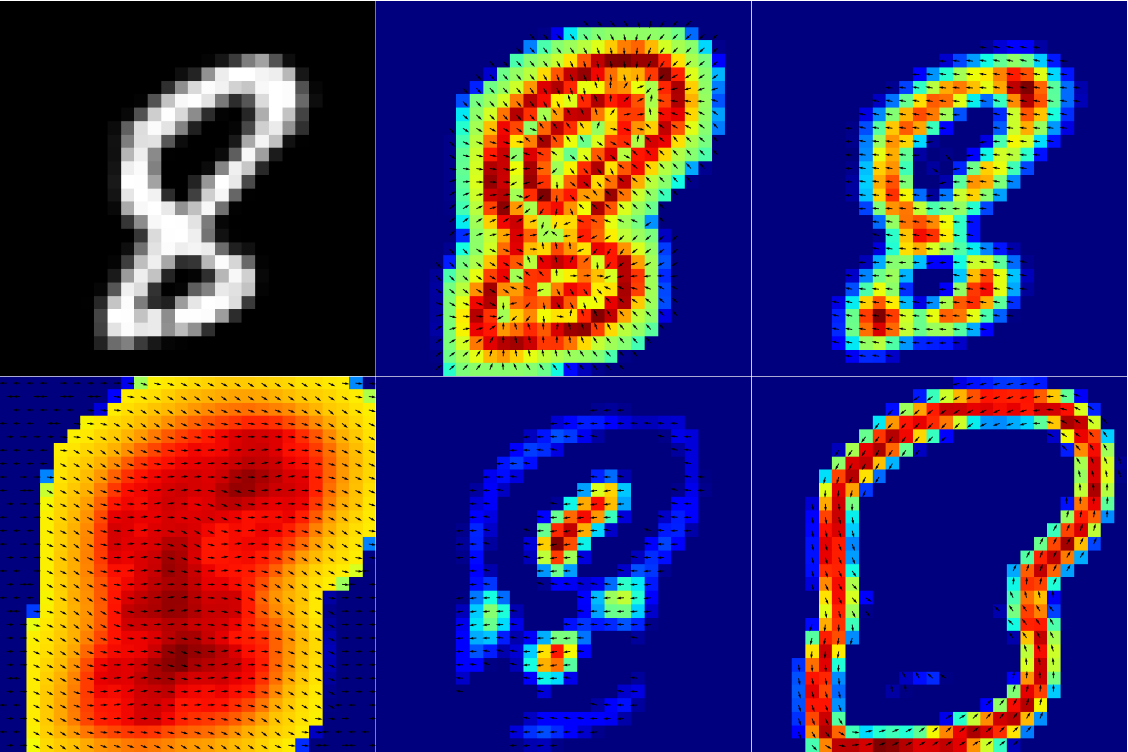
\includegraphics[scale=1]{images/fig10.png}\\
        Note: Arrows display phase
    \end{center}
}

\frame{
    \frametitle{Berkeley Segmentation Dataset (Boundary Detection)}
    \begin{center}
        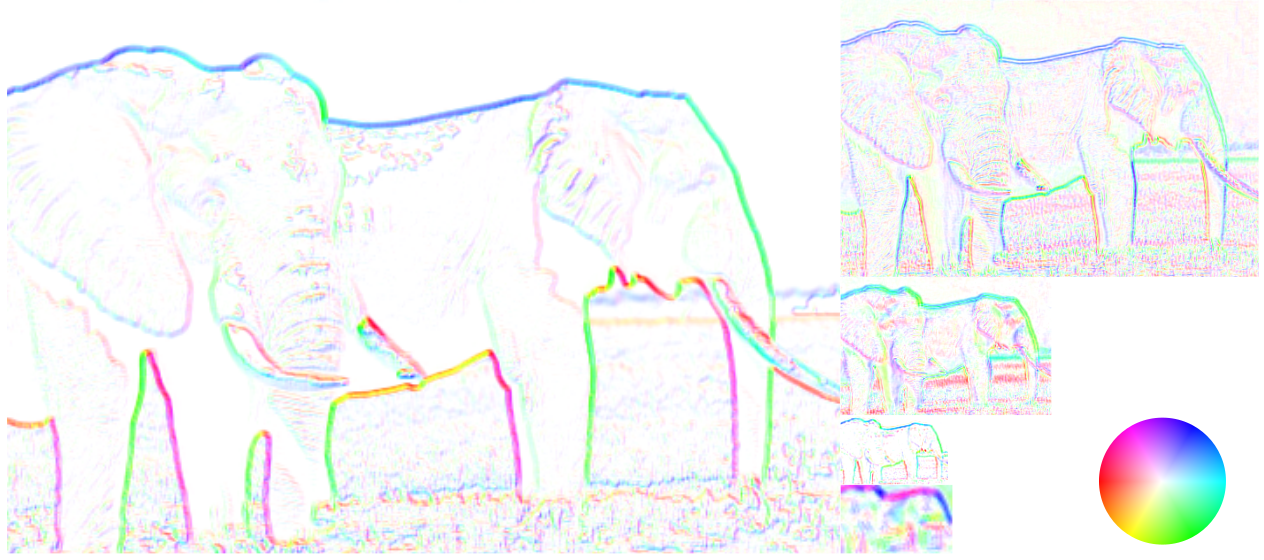
\includegraphics[scale=1]{images/fig11.png}\\
        \begin{tabular}{ |l|c|c|c| }
            \hline
            Method & ODS & OIS & \# Parameters\\
            \hline
            \hline
            Xie et al., & 0.64 & 0.65 & 2346k\\
            Kivinen et al., & 0.702 & 0.715 &-\\
            Harmonic Network & \textbf{0.726} & \textbf{0.742} & 116k\\ 
            \hline
        \end{tabular}
    \end{center}
}

\nocite{*} % Include everything in the .bib file.
\bibliographystyle{plainnat}
\bibliography{harmonic-networks}

% that's all, folks
\end{document}
